% Options for packages loaded elsewhere
\PassOptionsToPackage{unicode}{hyperref}
\PassOptionsToPackage{hyphens}{url}
%
\documentclass[
  11pt,
  spanish,
  oneside]{book}
\usepackage{amsmath,amssymb}
\usepackage[]{times}
\usepackage{ifxetex,ifluatex}
\ifnum 0\ifxetex 1\fi\ifluatex 1\fi=0 % if pdftex
  \usepackage[T1]{fontenc}
  \usepackage[utf8]{inputenc}
  \usepackage{textcomp} % provide euro and other symbols
\else % if luatex or xetex
  \usepackage{unicode-math}
  \defaultfontfeatures{Scale=MatchLowercase}
  \defaultfontfeatures[\rmfamily]{Ligatures=TeX,Scale=1}
\fi
% Use upquote if available, for straight quotes in verbatim environments
\IfFileExists{upquote.sty}{\usepackage{upquote}}{}
\IfFileExists{microtype.sty}{% use microtype if available
  \usepackage[]{microtype}
  \UseMicrotypeSet[protrusion]{basicmath} % disable protrusion for tt fonts
}{}
\makeatletter
\@ifundefined{KOMAClassName}{% if non-KOMA class
  \IfFileExists{parskip.sty}{%
    \usepackage{parskip}
  }{% else
    \setlength{\parindent}{0pt}
    \setlength{\parskip}{6pt plus 2pt minus 1pt}}
}{% if KOMA class
  \KOMAoptions{parskip=half}}
\makeatother
\usepackage{xcolor}
\IfFileExists{xurl.sty}{\usepackage{xurl}}{} % add URL line breaks if available
\IfFileExists{bookmark.sty}{\usepackage{bookmark}}{\usepackage{hyperref}}
\hypersetup{
  pdftitle={Manual para publicar un libro en GitHub creado en Bookdown},
  pdfauthor={Alvaro Martínez Rodríguez},
  pdflang={es},
  hidelinks,
  pdfcreator={LaTeX via pandoc}}
\urlstyle{same} % disable monospaced font for URLs
\usepackage[tmargin=2.5cm,bmargin=2.5cm,lmargin=2.5cm,rmargin=2.5cm]{geometry}
\usepackage{longtable,booktabs,array}
\usepackage{calc} % for calculating minipage widths
% Correct order of tables after \paragraph or \subparagraph
\usepackage{etoolbox}
\makeatletter
\patchcmd\longtable{\par}{\if@noskipsec\mbox{}\fi\par}{}{}
\makeatother
% Allow footnotes in longtable head/foot
\IfFileExists{footnotehyper.sty}{\usepackage{footnotehyper}}{\usepackage{footnote}}
\makesavenoteenv{longtable}
\usepackage{graphicx}
\makeatletter
\def\maxwidth{\ifdim\Gin@nat@width>\linewidth\linewidth\else\Gin@nat@width\fi}
\def\maxheight{\ifdim\Gin@nat@height>\textheight\textheight\else\Gin@nat@height\fi}
\makeatother
% Scale images if necessary, so that they will not overflow the page
% margins by default, and it is still possible to overwrite the defaults
% using explicit options in \includegraphics[width, height, ...]{}
\setkeys{Gin}{width=\maxwidth,height=\maxheight,keepaspectratio}
% Set default figure placement to htbp
\makeatletter
\def\fps@figure{htbp}
\makeatother
\setlength{\emergencystretch}{3em} % prevent overfull lines
\providecommand{\tightlist}{%
  \setlength{\itemsep}{0pt}\setlength{\parskip}{0pt}}
\setcounter{secnumdepth}{5}
\usepackage{booktabs}
\usepackage[utf8]{inputenc}
\usepackage[Glenn]{fncychap}
\pagestyle{plain}
\ifxetex
  % Load polyglossia as late as possible: uses bidi with RTL langages (e.g. Hebrew, Arabic)
  \usepackage{polyglossia}
  \setmainlanguage[]{spanish}
\else
  \usepackage[main=spanish]{babel}
% get rid of language-specific shorthands (see #6817):
\let\LanguageShortHands\languageshorthands
\def\languageshorthands#1{}
\fi
\ifluatex
  \usepackage{selnolig}  % disable illegal ligatures
\fi
\usepackage[]{natbib}
\bibliographystyle{plainnat}

\title{Manual para publicar un libro en GitHub creado en Bookdown}
\author{Alvaro Martínez Rodríguez}
\date{2022-01-07}

\begin{document}
\maketitle

{
\setcounter{tocdepth}{1}
\tableofcontents
}
\hypertarget{antes-de-empezar}{%
\chapter*{Antes de empezar}\label{antes-de-empezar}}
\addcontentsline{toc}{chapter}{Antes de empezar}

\hypertarget{cuenta-y-repositorio}{%
\section*{Cuenta y repositorio}\label{cuenta-y-repositorio}}
\addcontentsline{toc}{section}{Cuenta y repositorio}

Para poder hacer una publicación en \href{https://github.com/}{\textbf{Github}} es necesario crear una cuenta en esta plataforma. Para ello, hay que entrar en github.com y dar clic en \emph{Registrarse} y posteriormente entrar a la cuenta. Una vez dentro, en el lado superior izquierdo se encuentra el boton \emph{new} para crear un nuevo repositorio\footnote{Un repositorio es el sitio dentro del cual se alojarán los archivos del libro}.

\begin{figure}

{\centering 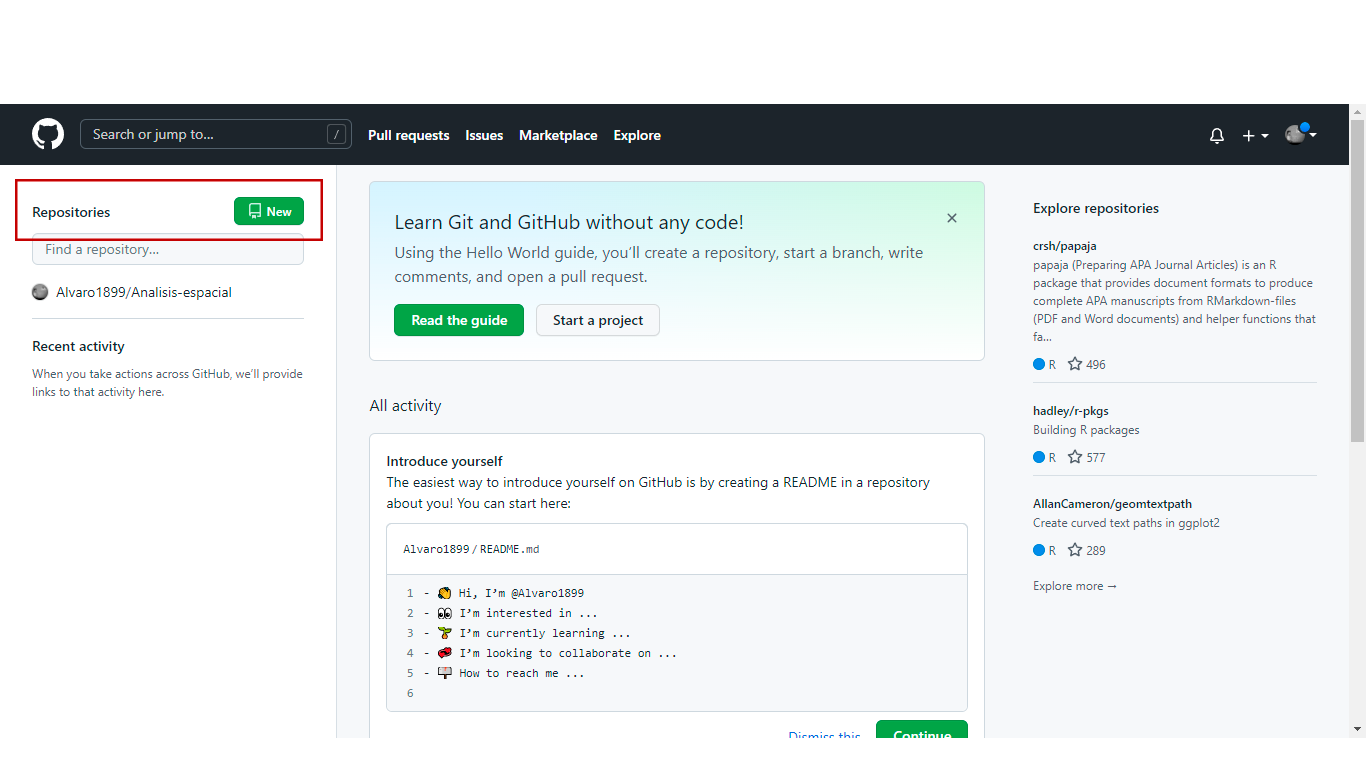
\includegraphics[width=1\linewidth]{imagenes/Imagen 1} 

}

\caption{.}\label{fig:unnamed-chunk-1}
\end{figure}

Para crear el repositorio solo es necesario darle un nombre y dar clic en el boton \emph{Crear repositorio}. Por ahora serà todo en GitHub, pero dejaremos la pagina abierta.

\begin{figure}

{\centering 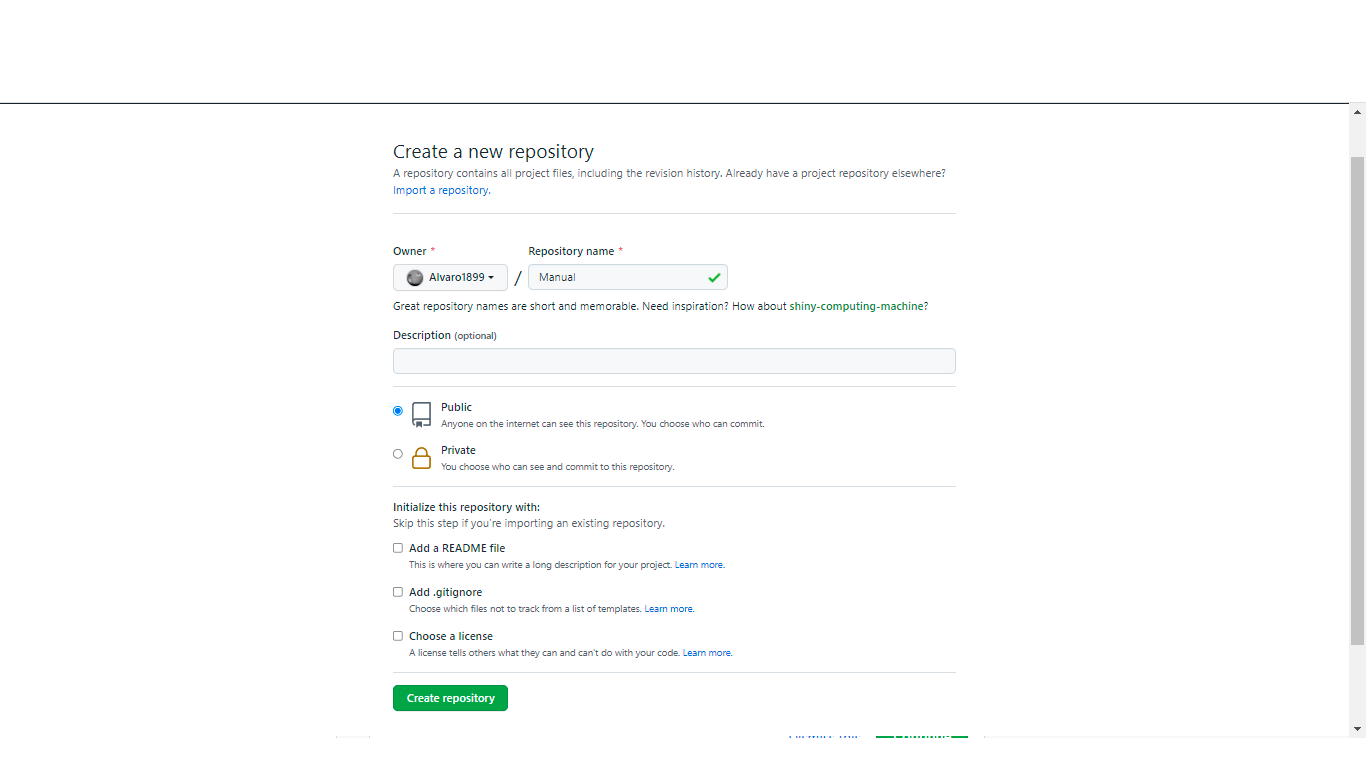
\includegraphics[width=1\linewidth]{imagenes/Imagen 2} 

}

\caption{.}\label{fig:unnamed-chunk-2}
\end{figure}

\hypertarget{programa-git}{%
\section*{Programa Git}\label{programa-git}}
\addcontentsline{toc}{section}{Programa Git}

Por otro lado tambien es necesario haber descargado \href{https://git-scm.com/}{Git}.Este programa nos ayudarà a enlazar R studio con GitHub. Damos clic en descargas para windows y después ejecutamos el archivo Git-2.34.1-64-bit.exe que se descargó para instalar Git.

\begin{figure}

{\centering 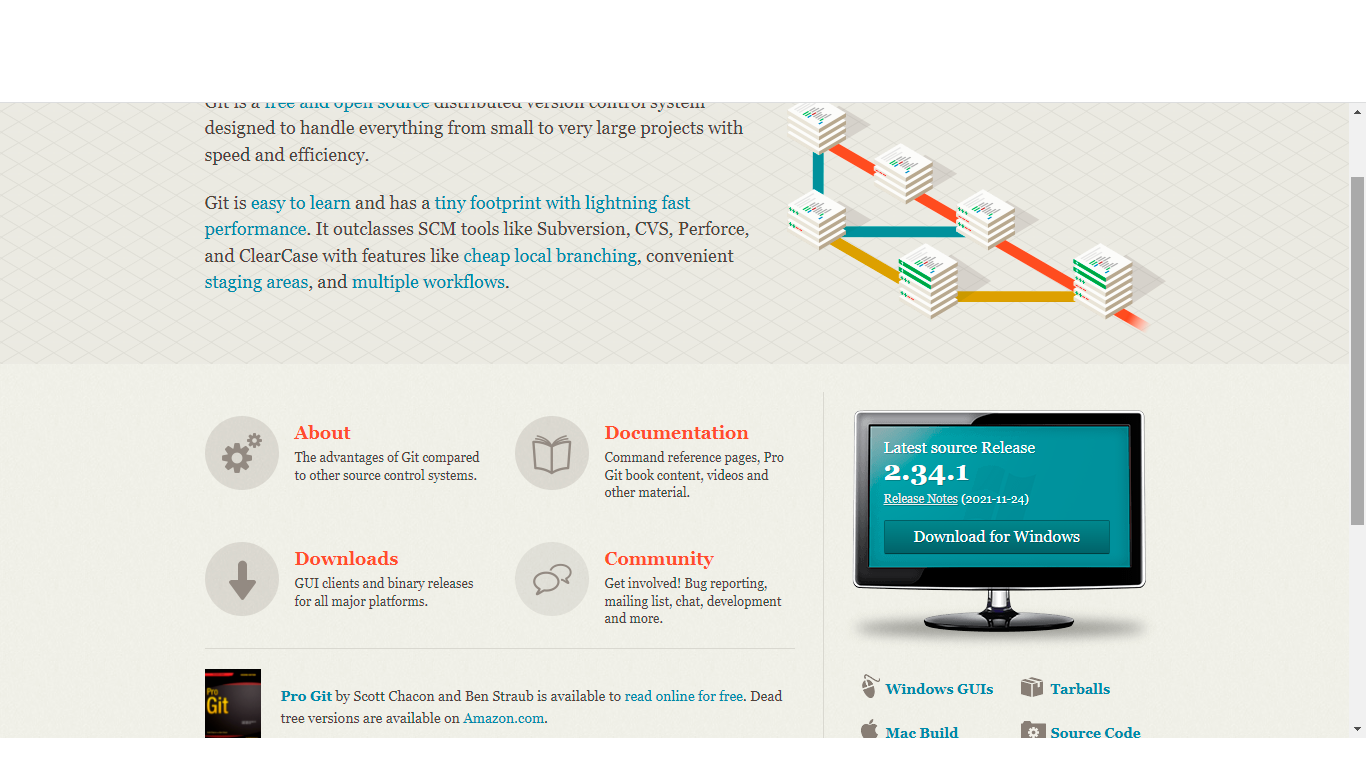
\includegraphics[width=1\linewidth]{imagenes/Imagen 3} 

}

\caption{.}\label{fig:unnamed-chunk-3}
\end{figure}

Por ùltimo, es necesario entrar en nuestro proyecto de R studio y seguimos los siguientes pasos.

Abrimos \emph{Tools} en la cinta de opciones -\textgreater{} \emph{Version Control} -\textgreater{} \emph{Project SetUp} -\textgreater{} Opciòn \emph{Git/SVN} -\textgreater{} Cambiamos la opciòn de \emph{control project system} de \textbf{None} a \textbf{Git}

\begin{figure}

{\centering 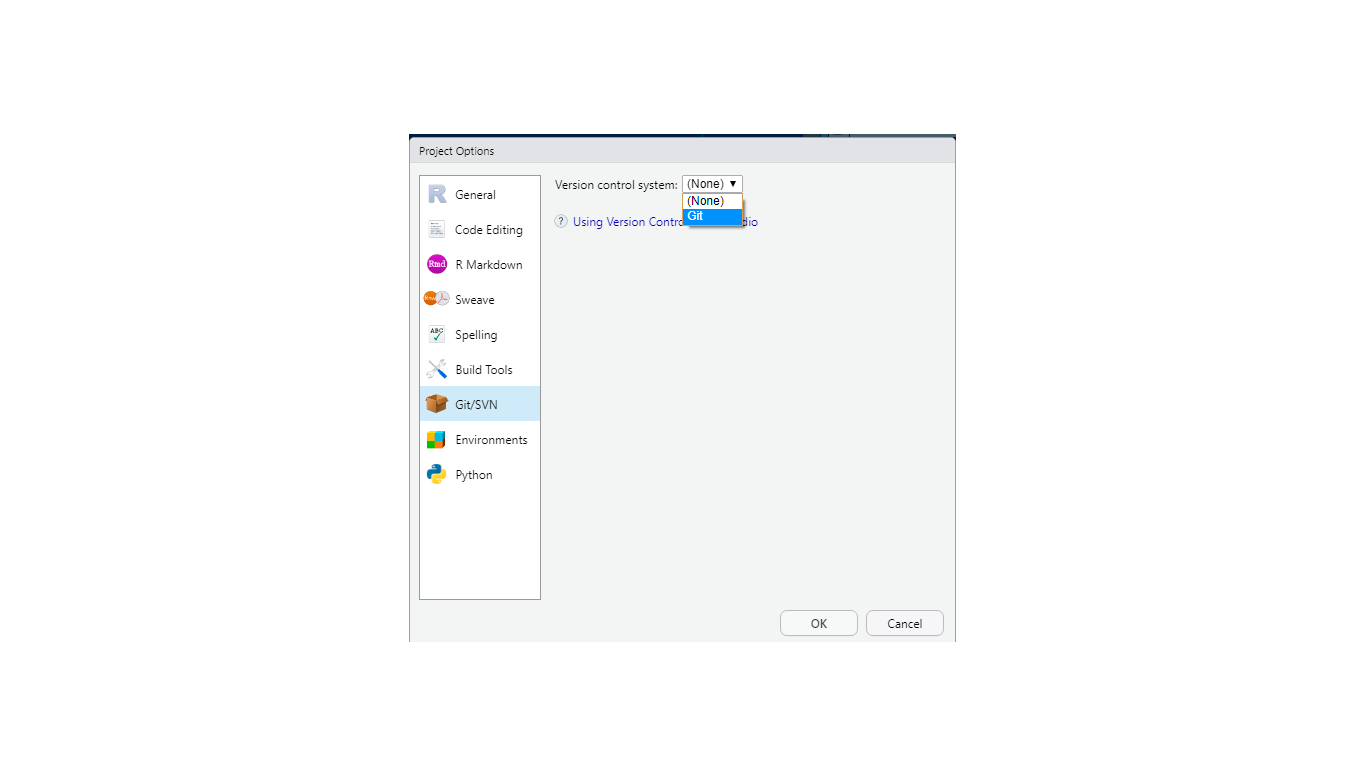
\includegraphics[width=1\linewidth]{imagenes/Imagen 4} 

}

\caption{.}\label{fig:unnamed-chunk-4}
\end{figure}

Después de realizar los pasos anteriores iremos a \emph{View} en la cinta de opciones y damos clic en \emph{Show Git}. Con ello nos aparecerá la pestaña Git que usaremos màs adelante.

\hypertarget{preparar-la-carpeta-del-proyecto}{%
\chapter*{Preparar la carpeta del proyecto}\label{preparar-la-carpeta-del-proyecto}}
\addcontentsline{toc}{chapter}{Preparar la carpeta del proyecto}

\hypertarget{carpeta-docs}{%
\section*{Carpeta docs}\label{carpeta-docs}}
\addcontentsline{toc}{section}{Carpeta docs}

Ahora, el siguiente paso es preparar la carpeta de nuestro proyecto. En este punto se espera que el lector ya haya construido el libro a través del boton \emph{Build Book} en formato \textbf{bookdown::github} o \textbf{bookdown::bs4\_book} de manera correcta.

En nuestra carpeta de proyecto debemos crear una carpeta con el nombre de \emph{docs}, en ella, GitHub podrà leer los archivos necesarios para el libro. Una vez creada, entraremos en la carpeta *\_book*. Aquí se encuentran los archivos renderizados en html de cada capitulo, así como todos los recursos que utilizan. Todos estos archivos los copiaremos y los pegaremos en la carpeta que creamos.

\begin{figure}

{\centering 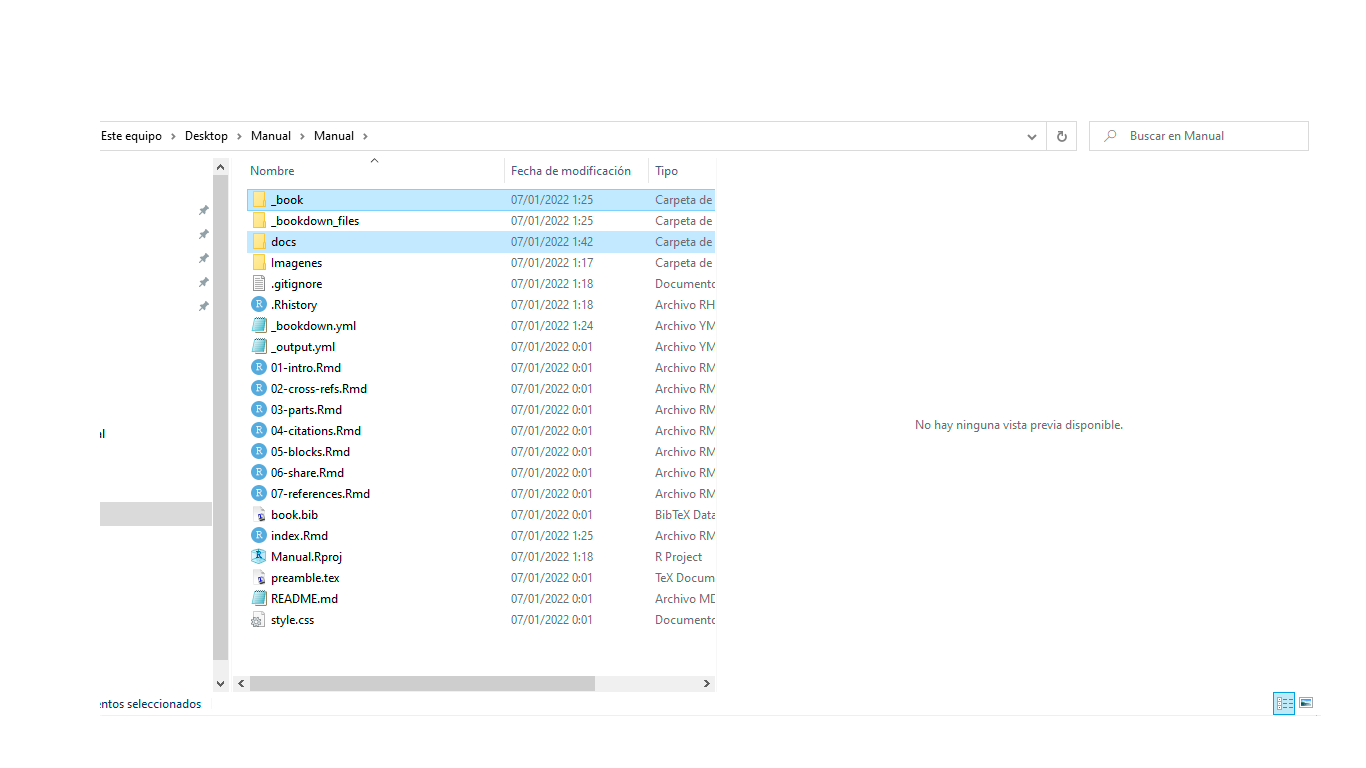
\includegraphics[width=1\linewidth]{imagenes/Imagen 5} 

}

\caption{.}\label{fig:unnamed-chunk-5}
\end{figure}

\hypertarget{archivos-de-texto}{%
\section*{Archivos de texto}\label{archivos-de-texto}}
\addcontentsline{toc}{section}{Archivos de texto}

Lo siguiente a realizar es la creación de 4 archivos: .nojekyll, .Rbuildignore, .travis.yml, DESCRIPTION

El primer archivo lo creáremos dentro de la carpeta \emph{docs} y para ello abriremos un nuevo archivo en R de tipo texto. No escribiremos nada en el archivo, solo lo guardamos con el nombre \textbf{.nojekyll}

\emph{File} -\textgreater{} \emph{New File} -\textgreater{} \emph{Text File}

Volvemos a crear un archivo de texto, escribimos el siguiente codigo dentro y lo guardamos en la carpta principal con el nombre \textbf{.Rbuildignore}

\begin{figure}

{\centering 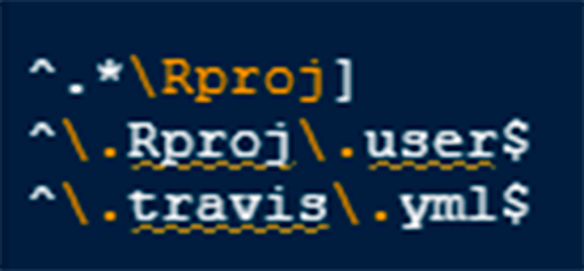
\includegraphics[width=0.7\linewidth]{imagenes/Imagen 6} 

}

\caption{.}\label{fig:unnamed-chunk-6}
\end{figure}

Ahora creamos otro archivo de texto con el siguiente codigo y lo guardamos con el nombre .travis.yml

\begin{figure}

{\centering 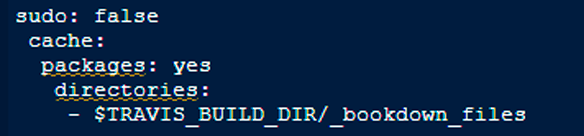
\includegraphics[width=0.7\linewidth]{imagenes/Imagen 7} 

}

\caption{.}\label{fig:unnamed-chunk-7}
\end{figure}

Por ùltimo creamos otro archivo con el nombre de \textbf{DESCRIPTION} y escribimos lo siguiente:

\begin{figure}

{\centering 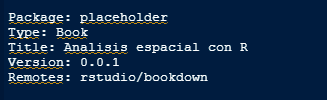
\includegraphics[width=0.7\linewidth]{imagenes/Imagen 8} 

}

\caption{.}\label{fig:unnamed-chunk-8}
\end{figure}

\hypertarget{subida-de-archivos}{%
\chapter*{Subida de archivos}\label{subida-de-archivos}}
\addcontentsline{toc}{chapter}{Subida de archivos}

\hypertarget{vinculaciuxf2n}{%
\section*{Vinculaciòn}\label{vinculaciuxf2n}}
\addcontentsline{toc}{section}{Vinculaciòn}

Hasta ahora hemos preparado nuestro proyecto para poderlo subir de manera correcta. Iremos a R studio para comenzar a subir los archivos. En la pestaña de \emph{Git} y en el botón de engrane seleccionaremos la opción \emph{Shell}. Se abrirá una ventana cmd, en ella, deberemos copiar el código que aparece en nuestro repositorio creado de GitHub. Esto permitirà que Rstudio y GitHub este conectados y le indicara a R en donde debe subir los archivos.

\begin{figure}

{\centering 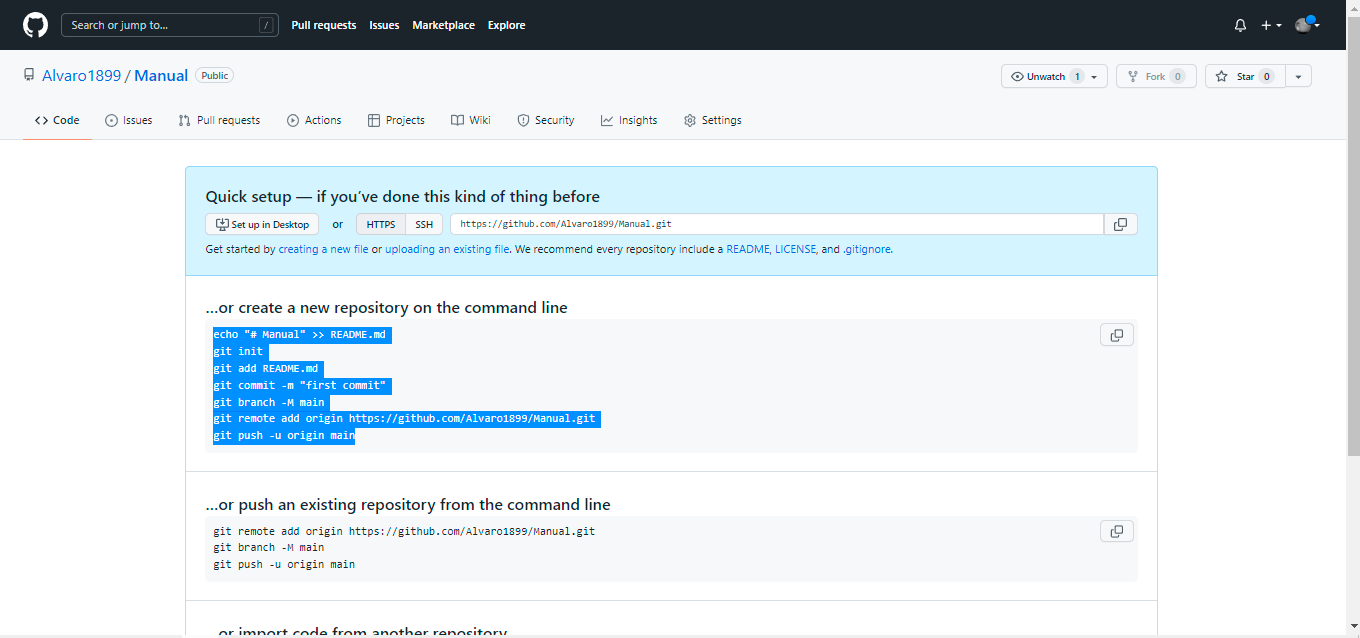
\includegraphics[width=0.7\linewidth]{imagenes/Imagen 9} 

}

\caption{.}\label{fig:unnamed-chunk-9}
\end{figure}

\begin{figure}

{\centering 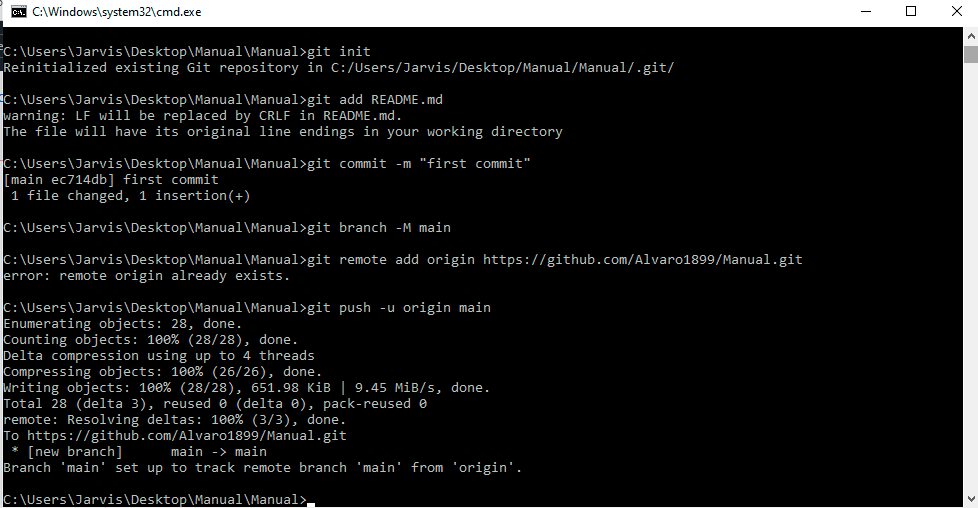
\includegraphics[width=0.7\linewidth]{imagenes/Imagen 11} 

}

\caption{Resultado de pegar el codigo}\label{fig:unnamed-chunk-10}
\end{figure}

Cerramos la ventana de sistema cmd y regresamos a Rstudio. En la misma pestaña de Git nos aparecerán una serie de archivos que contiene nuestro libro y deberemos seleccionarlos todos dando clic en la columna de \emph{Staged}\footnote{En ocaciones, despues de dar clic en el recuadro blanco tarda unos segundos en marcarlo, por lo que deberemos ser pacientes y no dar mas de un clic por archivo.}.

\begin{figure}

{\centering 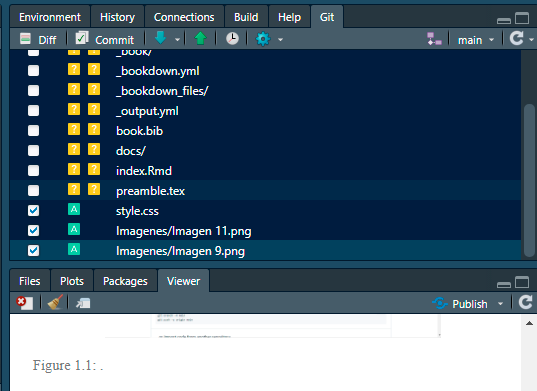
\includegraphics[width=0.7\linewidth]{imagenes/Imagen 10} 

}

\caption{.}\label{fig:unnamed-chunk-11}
\end{figure}

Presionaremos el botón de \emph{Commit} y escribiremos en el recuadro derecho ``Subida de archivos'' y daremos clic en el botón \emph{Commit}. Una vez termine el proceso resultante de paso anterior daremos clic en la flecha verde \emph{Push} que esta en la parte superior derecha y esperaremos a que se suban los archivos.

\begin{figure}

{\centering 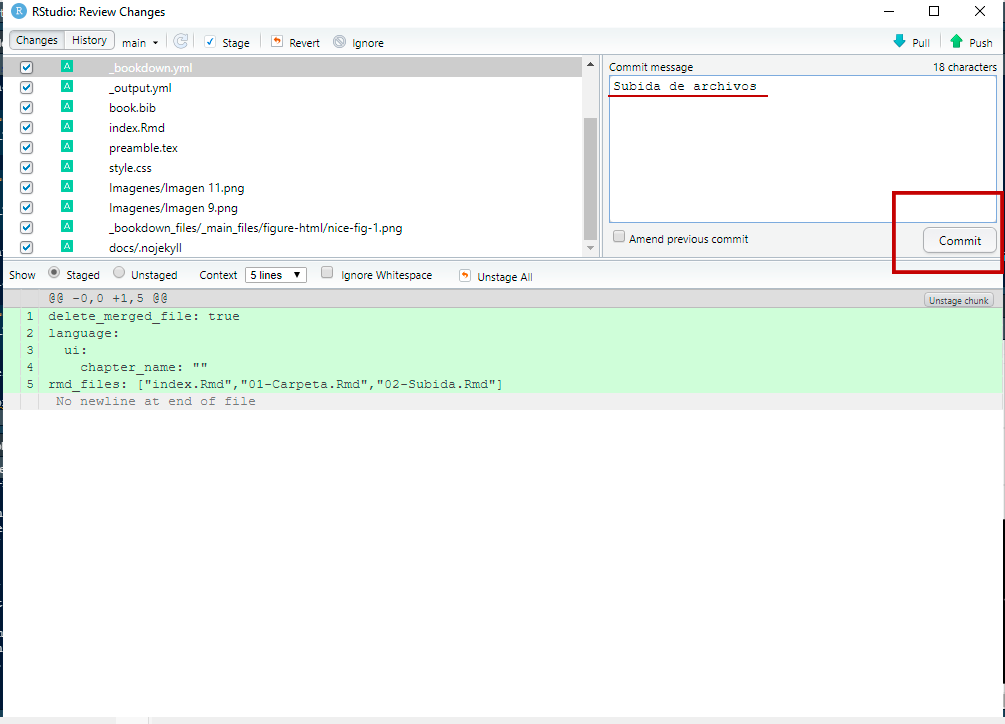
\includegraphics[width=0.7\linewidth]{imagenes/Imagen 12} 

}

\caption{.}\label{fig:unnamed-chunk-12}
\end{figure}

\begin{figure}

{\centering 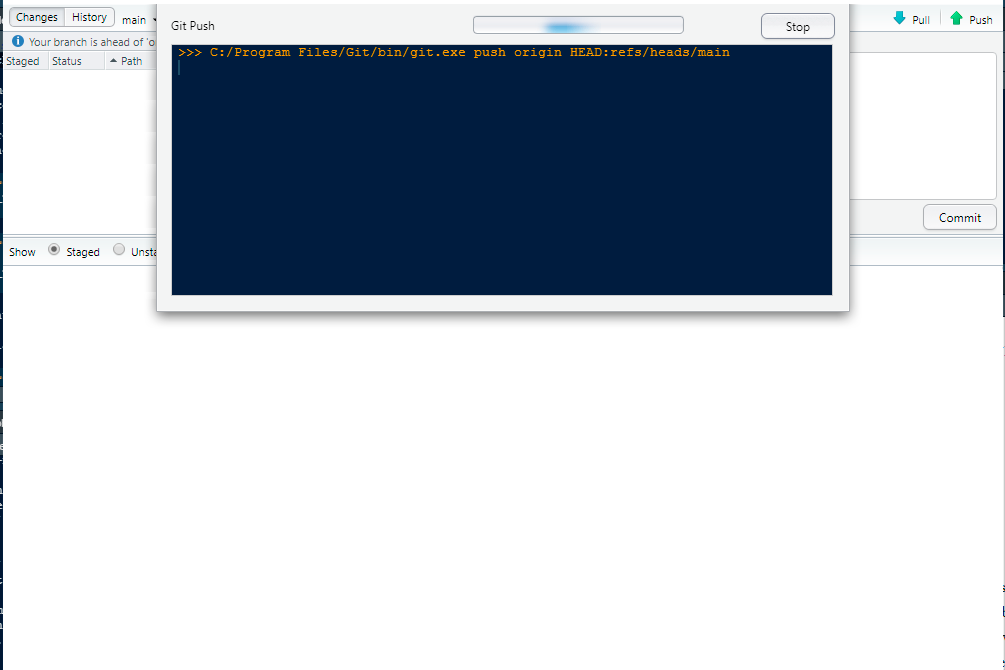
\includegraphics[width=0.7\linewidth]{imagenes/Imagen 13} 

}

\caption{Resultado final de *Push*}\label{fig:unnamed-chunk-13}
\end{figure}

Ahora ya tenemos nuestros archivos subidos en nuestro repositorio de GitHub.

\hypertarget{link}{%
\section*{Link}\label{link}}
\addcontentsline{toc}{section}{Link}

Para obtener el link del documento que acabamos de publicar debemos ir a nuestro repositorio en GitHub. Una ves dentro, podremos observar en la pantalla principal todos los archivos que se han subido de nuestro libro. Daremos clic en \emph{Settings}

\begin{figure}

{\centering 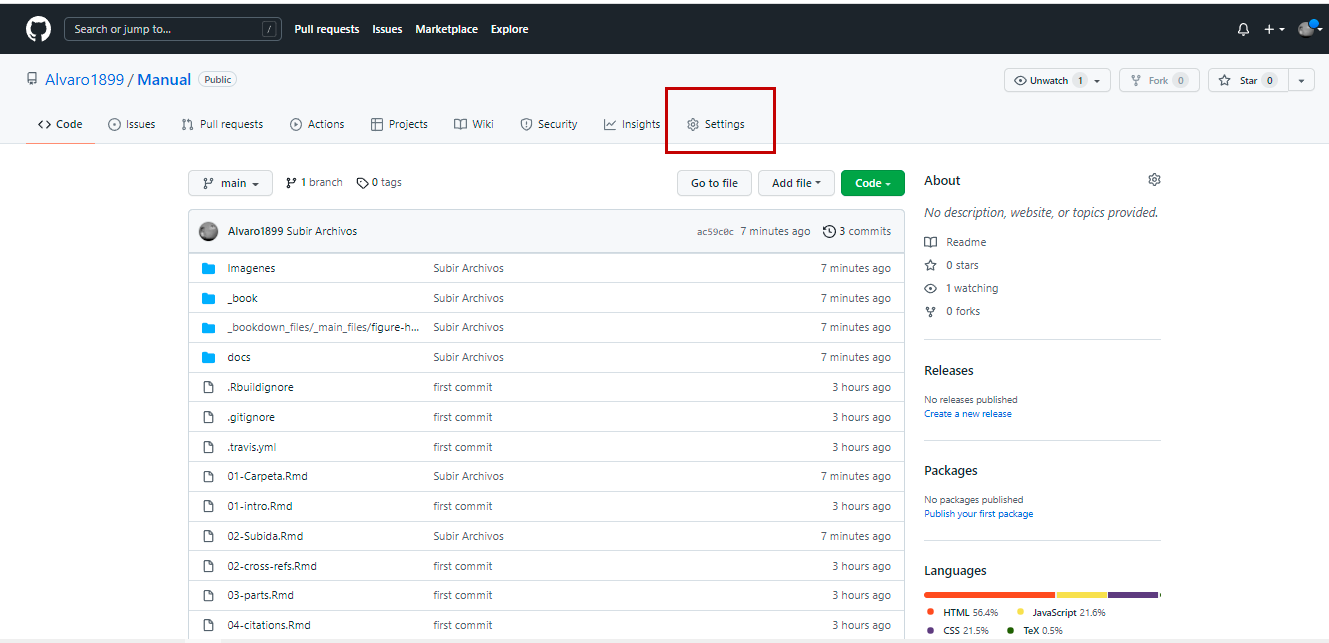
\includegraphics[width=0.7\linewidth]{imagenes/Imagen 14} 

}

\caption{.}\label{fig:unnamed-chunk-14}
\end{figure}

Dentro de \emph{Settings} nos aparecerá un menú a la izquierda, en donde seleccionaremos la opción de \emph{Pages}. En este apartado tenemos la sección de \emph{Source}, ahì debemos cambiar la opciòn \textbf{None} por la rama \textbf{Main} y la carpeta \textbf{Docs} y lo guardamos con el botón \emph{Save}. Una vez lo anterior, nos aparecerá en la parte de arriba el link de nuestro documento publicado.

\begin{figure}

{\centering 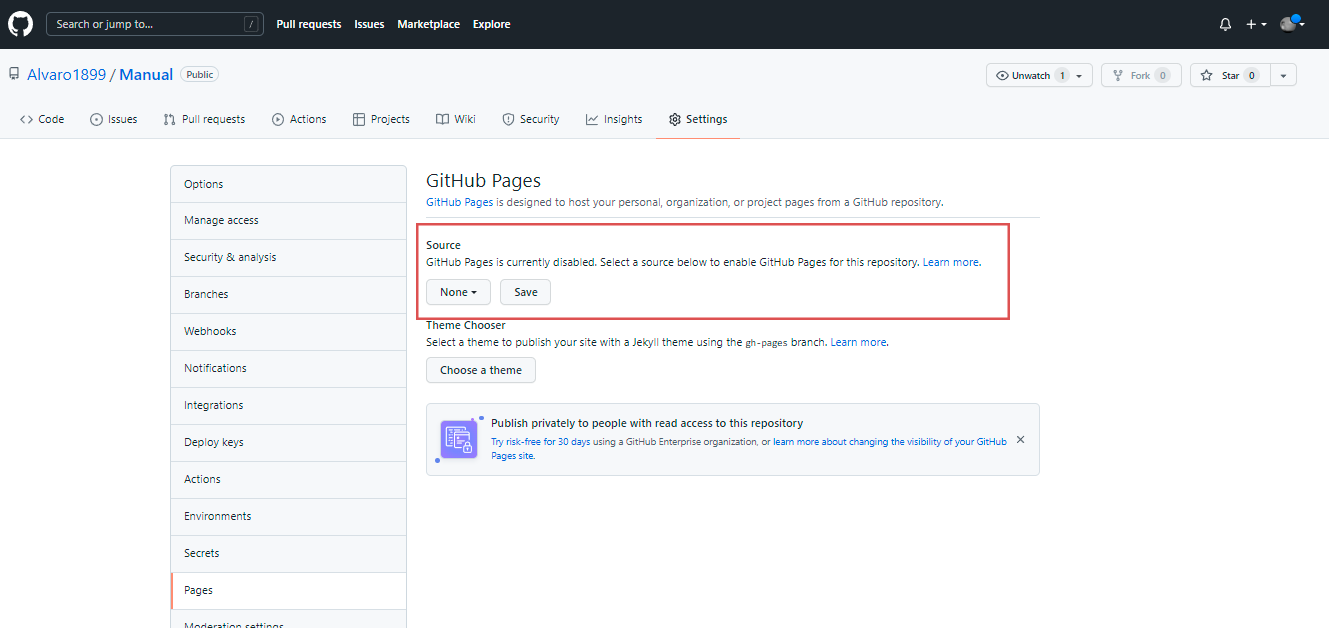
\includegraphics[width=0.7\linewidth]{imagenes/Imagen 15} 

}

\caption{.}\label{fig:unnamed-chunk-15}
\end{figure}

\begin{figure}

{\centering 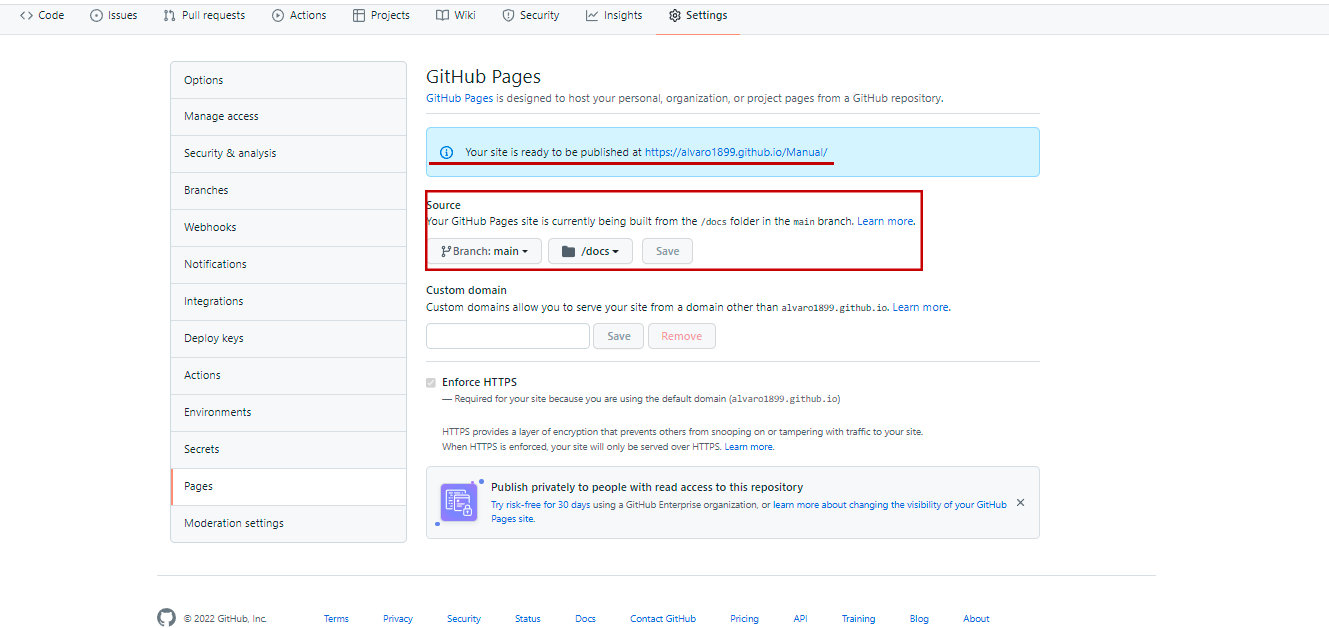
\includegraphics[width=0.7\linewidth]{imagenes/Imagen 16} 

}

\caption{.}\label{fig:unnamed-chunk-16}
\end{figure}

\hypertarget{actualizaciuxf2n}{%
\chapter*{Actualizaciòn}\label{actualizaciuxf2n}}
\addcontentsline{toc}{chapter}{Actualizaciòn}

Para actualizar nuestro libro solo hace falta volverlo a correr en formato \textbf{bookdown::github} o \textbf{bookdown::bs4\_book}. Esto generara automáticamente los archivos en la carpeta *\_book\emph{. Copiamos los archivos generados en }docs\emph{, vamos a la carpeta Git en R, seleccionamos todos los archivos que aparezcan, entramos en }Commit\emph{, escribimos ``Actualizaciòn'', presionamos en }Commit* de nuevo y despuès en \emph{Push}. Verificamos que se hayan actualizado los documentos en GitHub.

  \bibliography{book.bib}

\end{document}
